To start using the nonlinear static procedure with record-to-record variability a command line text editor should be used to enter manually the folder location where the \textit{rmtk} has been saved, as shown in the example below:

\begin{Verbatim}[frame=single, commandchars=\\\{\}, samepage=true]
~\$ cd path/to/rmtk/folder/rmtk/vulnerability
\end{Verbatim}

Where /path/to/rmtk/folder/ is the system path to the location of the \textit{rmtk} folder. From the text editor iPython browser page can be opened with the following command line:

\begin{Verbatim}[frame=single, commandchars=\\\{\}, samepage=true]
~\$ ipython-2.7 notebook --pylab=inline
\end{Verbatim}

Once the iPython page is opened on the browser, the python scripts contained in the \textit{vulnerability} directory will be visible. The file \textit{NSM\_dispersion.ipynb} should be selected to start the calculations.

In the initial section of the script "Define Options" the user should set the options, while the input corresponding to the defined options should be entered in the folder \textit{NSP/input}. The main options to define are the following:

\begin{itemize}
\item Type of procedure to perform: either C$_R$-based, spo2ida-based or R-$\mu$-T-based. The main difference between the three is that C$_R$-based procedure is applicable to elasto-plastic idealised capacity curve only, while spo2ida-based and R-$\mu$-T-based procedure fit any kind of multilinear curve. Among the two procedures for multilinear capacity curves the main difference lies in the spo2ida-based ability to compute more accurately the record-to-record dispersion. 
\item Type of input: either results of a pushover analysis in terms of displacement vs base shear at each time step or idealised pushover curve, as shown in Figures \ref{fig:expPushover} and \ref{fig:expIdealised}.

\begin{figure}[!htbp]
\centering
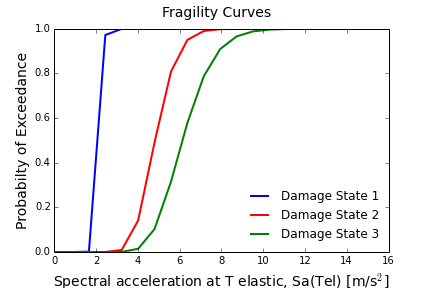
\includegraphics[width=10cm]{./figures/PushoverCurve.png}
\caption{Pushover curve.}
\label{fig:expPushover}
\end{figure}

\begin{figure}[!htbp]
\centering
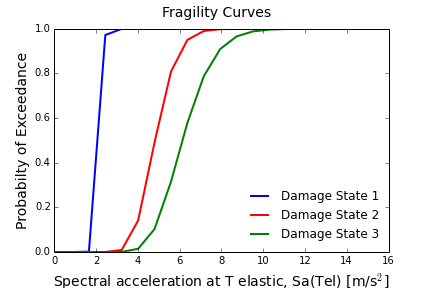
\includegraphics[width=10cm]{./figures/IdealisedCurve.png}
\caption{Idealised pushover curve.}
\label{fig:expIdealised}
\end{figure}

\item Type of output: either fragility curve (probability of exceedance of a set of limit states vs seismic intensity, as shown in Figure \ref{fig:expFragility}) or vulnerability curve (loss ratio vs seismic intensity, as shown in Figure \ref{fig:expVulnerability}).
\end{itemize}

\begin{figure}[!htbp]
\centering
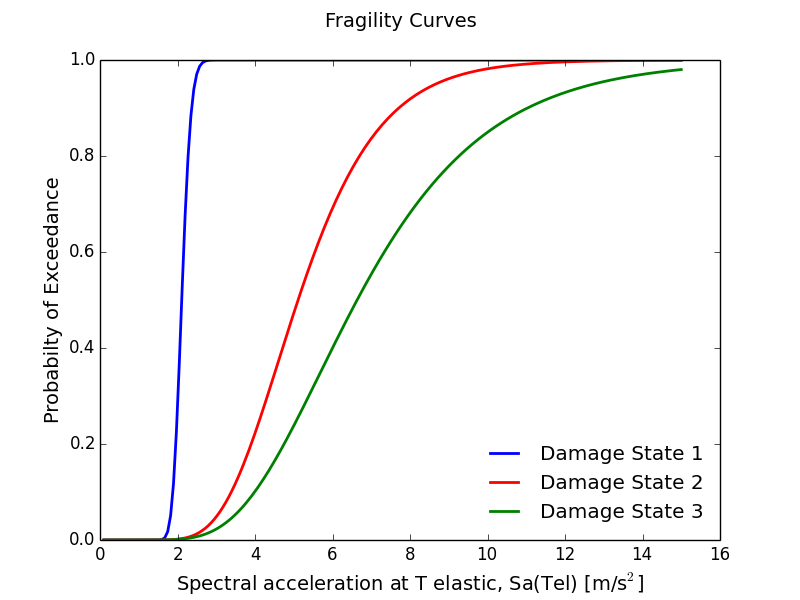
\includegraphics[width=10cm]{./figures/fragility.png}
\caption{Output: fragility curve}
\label{fig:expFragility}
\end{figure}

\begin{figure}[!htbp]
\centering
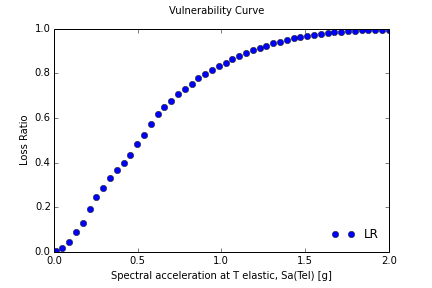
\includegraphics[width=10cm]{./figures/vulnerability.png}
\caption{Output: vulnerability curve}
\label{fig:expVulnerability}
\end{figure}

The outputs could be found in the \textit{outputs} folder, located in the \textit{vulnerability} directory. The nonlinear static procedure with dispersion produces results in terms of spectral acceleration in units of g. Therefore the mean spectral acceleration of the lognormal fragility curves and the spectral acceleration levels corresponding to each loss ratio in the vulnerability curve are in units of g.
These options and others need to be defined in the initial section of the script "Define Options". In section \ref{subsubsec:options} the alternatives values that the initial variables can assume and their meaning are described in detail, while the parameters to be inserted in the input files are listed below. They are fully described in section \ref{subsec:nls-ruiz-garcia-miranda} section \ref{subsec:nls-spo2ida} and section  \ref{subsec:nls-dolsek-fajfar}, within the presentation of each of the three procedures.

\subsubsection{Options}
\label{subsubsec:options}
The type of procedure to be performed and the type of inputs at disposal, are set with the variables \textit{an\_type} and \textit{in\_type} respectively. With the variable \textit{an\_type} the user can choose between:

\begin{Verbatim}[frame=single, commandchars=\\\{\}, samepage=true]
an\_type = 0 #Cr-based procedure (Ruiz-Garcia and Miranda, 2007)
an\_type = 1 #spo2ida-based procedure (Vamvatsikos and Cornell, 2006)
an\_type = 2 #R-m-T-based procedure (Dolsek and Fajfar, 2004)
\end{Verbatim}

With the variable \textit{in\_type} the user can choose between:

\begin{Verbatim}[frame=single, commandchars=\\\{\}, samepage=true]
in\_type = 0 # idealised pushover curve
in\_type = 1 # raw results from a pushover analysis
\end{Verbatim}

The variable \textit{vuln} instead gives the opportunity to decide the type of outputs, whether to stop the process at the derivation of the fragility curves, or to go all the way up to the vulnerability curve definition, applying damage-to-loss functions.

\begin{Verbatim}[frame=single, commandchars=\\\{\}, samepage=true]
vuln = 0 # derive fragility curves 
vuln = 1 # derive vulnerability curve
\end{Verbatim}

The variable \textit{g} serves the purpose of defining the units that are being used. A floating number must be assigned to the gravity acceleration, compatible with the units used for the period of vibration and for the displacements (if the period is expressed in seconds and displacements are in meters, then g = 9.81). The variable \textit{iml} is a numpy array that identifies the intensity measure levels for which loss ratios are computed and provided in the vulnerability curve. The variable \textit{MC} fix the number of Monte Carlo simulations to account for uncertainty in damage thresholds.

\begin{Verbatim}[frame=single, commandchars=\\\{\}, samepage=true]
g = 9.81
iml = np.linspace(0.1,15,100)
MC = 25
\end{Verbatim}

The variable \textit{plotflag} allows or inhibits the displaying of plots. It is a python list composed of 4 integers, each one controlling a different plot: idealised pushover curve, 16\%-50\%-84\% ida curves, fragility curves and vulnerability curve respectively. Each integer can take as value either zero or one, whether the corresponding graph has to be displayed or not:

\begin{Verbatim}[frame=single, commandchars=\\\{\}, samepage=true]
plotflag = [1, 1, 1, 1] # plot all the graphs
plotflag = [0, 0, 0, 0] # do not plot any graph
\end{Verbatim}

The following variables set some of the characteristics of the plots:

\begin{itemize}
\item \textit{linew}: integer for defining lines width.
\item \textit{fontsize}: fontsize used for labels, graphs etc.
\item \textit{units}: list of 3 strings defining displacements, forces and Spectral acceleration units, as ['[kN]', '[m]', '[m/s$^2$]'], to be displayed on the axes of the plots.
\end{itemize}

The variable \textit{N} is needed for spo2ida-based procedure only and it represents the number of points per segment of IDA curve derived with spo2ida.

The last set of variables is needed for R-$\mu$-T-based procedure only:
\begin{itemize}
\item \textit{Tc}: constant accel-constant velocity corner period of a Newmark-Hall type spectrum. Default value is 0.5.
\textit{Td}: constant velocity-constant displacement corner period of a Newmark-Hall type spectrum. Default value is 1.8.
\end{itemize}
